
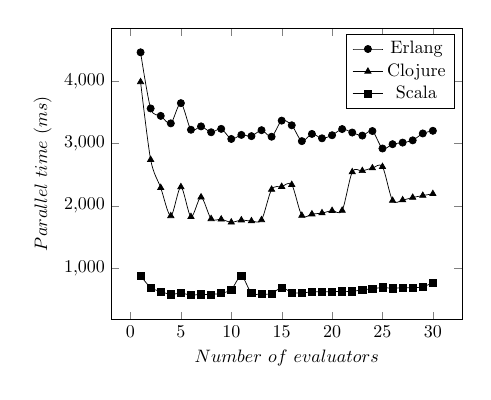
\begin{tikzpicture}[thick, scale=0.65]

  \begin{axis}[
         xlabel=$Number \hspace{.12cm} of \hspace{.12cm} evaluators$,
         ylabel=$Parallel \hspace{.12cm} time \hspace{.12cm} (ms)$
         ]
     \addplot[smooth,mark=*]  plot coordinates{
(1,4466.6)
(2,3564.222222222222)
(3,3444.6666666666665)
(4,3324.5555555555557)
(5,3649.6)
(6,3221.7)
(7,3275.9)
(8,3181.3)
(9,3236.0)
(10,3073.5555555555557)
(11,3139.0)
(12,3119.1111111111113)
(13,3214.9)
(14,3109.5555555555557)
(15,3368.3)
(16,3293.7)
(17,3039.1)
(18,3154.7)
(19,3084.1)
(20,3133.6666666666665)
(21,3232.9)
(22,3177.1111111111113)
(23,3128.0)
(24,3201.3333333333335)
(25,2920.4)
(26,2989.5555555555557)
(27,3015.4)
(28,3051.4444444444443)
(29,3162.3)
(30,3204.7)
     };
     \addlegendentry{Erlang}

     \addplot[smooth,mark=triangle*]
         plot coordinates{
(1,3990.75)
(2,2740.777777777778)
(3,2289.1111111111113)
(4,1837.111111111111)
(5,2302.5555555555557)
(6,1822.6666666666667)
(7,2138.6666666666665)
(8,1789.5)
(9,1782.3333333333333)
(10,1734.6666666666667)
(11,1768.888888888889)
(12,1754.7777777777778)
(13,1772.0)
(14,2261.1111111111113)
(15,2307.8888888888887)
(16,2338.4444444444443)
(17,1842.3333333333333)
(18,1865.7777777777778)
(19,1883.4444444444443)
(20,1920.7777777777778)
(21,1923.5)
(22,2542.1111111111113)
(23,2561.6666666666665)
(24,2605.5555555555557)
(25,2627.0)
(26,2083.0)
(27,2091.8888888888887)
(28,2132.222222222222)
(29,2163.777777777778)
(30,2192.1111111111113)
         };
     \addlegendentry{Clojure}


     \addplot[smooth,mark=square*]
         plot coordinates{
(1,876.6666666666666)
(2,683.7777777777778)
(3,622.2857142857143)
(4,575.2222222222222)
(5,596.0)
(6,563.0)
(7,576.2222222222222)
(8,574.0)
(9,595.1111111111111)
(10,651.8888888888889)
(11,871.6666666666666)
(12,595.3333333333334)
(13,582.25)
(14,586.8888888888889)
(15,684.8888888888889)
(16,605.0)
(17,600.625)
(18,614.0)
(19,618.2222222222222)
(20,616.7777777777778)
(21,625.2222222222222)
(22,622.6666666666666)
(23,649.7777777777778)
(24,664.1111111111111)
(25,686.625)
(26,672.4444444444445)
(27,684.7777777777778)
(28,681.625)
(29,698.0)
(30,760.7142857142857)
         };
     \addlegendentry{Scala}

  \end{axis}

\end{tikzpicture}

